\chapter{Results}

\label{Chapter5}

Results for both structured and statistical implementations presented in Chapter \ref{Chapter3}, are applied to a set of corpora in order to be evaluated. \par

\section{Structural Approach}

The structural approach described in previous chapters is being assessed into this section. For this purpose, the code of Appendix \ref{Appendix8} alongside with two IBM corpora was applied. It has to be mentioned that these two IBM corpora include only argumentative sentences, and we aim to check how many of those arguments will be identified correctly by our algorithm. 

The metric of accuracy was used in order to evaluate the indicators selected for recognizing argumentative sentences, while precision, recall and f1 score did not have value because of the non-arguments lack. For measuring accuracy, four counters were used; \textbf{true positives} (tp) is counting the times both algorithm and analyst labeled a sentence as argumentative, \textbf{true negatives} (tn) how often both algorithm and analyst labeled as non-argumentative, \textbf{false positive} (fp) the times the algorithm assigned as argumentative a sentence that expert recognized as non-argumentative, \textbf{false negative} (fn) how many times human identified a sentence as argumentative while algorithm did not. 

\begin{itemize}
 	\item \textbf{Accuracy} represents the percentage of correctly classified sentences:
 	\[ A
 	= \dfrac{tp + tn}{tp + tn + fp + fn}
 	\]
 	\item \textbf{Precision} indicates the times of correctly identification instances:
 	\[ P
 	= \dfrac{tp}{tp + fp}
 	\]
 	\item \textbf{Recall} measures the times algorithm missed out arguments:
 	\[ R
 	= \dfrac{tp}{tp + fn}
 	\]
 	\item \textbf{F1 Score} presents the mean of precision and recall:
 	\[ F
 	= \dfrac{2*P*R}{P + R}
 	\]
\end{itemize} 

\begin{table}[H]
	\centering
	\resizebox{0.65\linewidth}{!}{%
	\begin{tabular}{ | p{2cm} |  p{4cm} | p{2cm} | }
		\hline
		\textbf{Source Data} 
				& \textbf{file} 			
						& \textbf{Accuracy}  		\\[0.5cm] \hline
										
		\cite{bar-haim-etal-2017-stance}
				&claim\_stance\_dataset\_v1
						&17.50\%					\\[0.2cm] 
		\cite{Aharoni2014}
				&CDEdata.xls1.00.1480.25
						&14.81\%					\\[0.2cm]
		\hline
	\end{tabular}}
	\caption{Results of Structural Approach} 
	\label{structural_approach_results}
\end{table}

Structural approach seems not to be able to capture a variety of argumentative structures. This is beacause, argumentative patterns are rarely used in practice, since human discourse involves a lot of information which is being implied rather than being explicitly stated.

\newpage
\section{Statistical Approach}

\subsection{Random Forest Algorithm}
Supervised machine learning algorithms need a number of labeled data in order to be trained. That was the reason corpora of Chapter \ref{Chapter4} was created, and used in the implantation of Random Forest classifier algorithm (Appendix \ref{Appendix9}). A number of 33\% of the data used to train the model, while the rest of them to evaluate the results. 

It has to be mentioned that two methods were used for argument's classification. The first one was by tokenizing the sentences, so as to be in a format that a computer can understand, and then training the model based on the tokenized sentences. This method had an accuracy of \textbf{56.83\%}, precision \textbf{100\%}, recall \textbf{0.55\%}, f1 score \textbf{71.13\%}, and the results are displayed in the heatmap of figure \ref{random_forest} (A). Based on the results, it seems that Random Forest trained by tokenized sentencses is not recognizing argumentative sentences. That's why we implemented another technique in which we determined some features of each sentence ,and then feed the algorithm with these features instead of the sentences. In this way the accuracy increased to \textbf{79.42\%}, while precision is \textbf{74.08\%}, recall \textbf{78.72\%}, f1 score \textbf{76.33\%} , and it deprecates to the heatmap of figure \ref{random_forest} (B). The results of the first approach are not that high, and that is probably because of the unique words.

The features used for classification are the following based on the paper (\cite{Lawrence2016}):

\begin{itemize}
	\item \textbf{Word Counter}: the number of words in a sentence
	\item \textbf{Uppercase Characters Counter}: the number of uppercase characters found
	\item \textbf{Punctuation or Special Characters Counter}: the number of presence punctuation characters like " "
\end{itemize} 

\begin{figure}[H]
	\centering
	\subfloat[Classification based 
	on the sentences]{{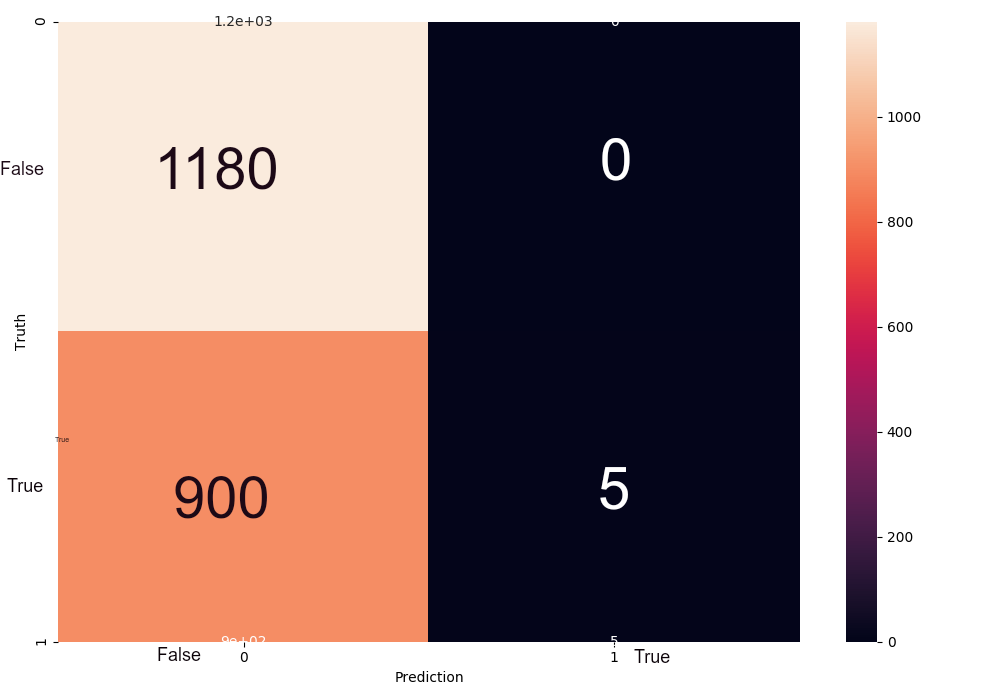
\includegraphics[scale=0.2]{images/random_forest_sentences.png} }}%
	\qquad
	\subfloat[Classification based 
	on features]{{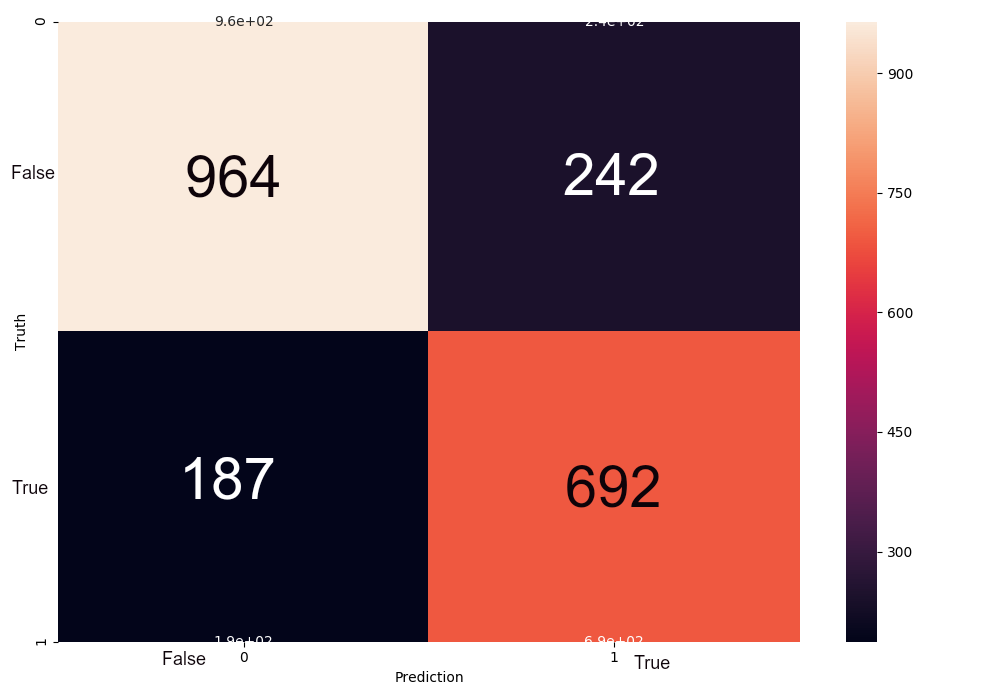
\includegraphics[scale=0.2]{images/random_forest_features.png} }}%
	\caption{
		Predicted and Real results of Random Forest classification algorithm
	}
	\label{random_forest}
\end{figure}

As the results of table \ref{random_forest} reveal, Random Forest implements well when features are used for each of sentence. Machine learning approach seems to be a better fit for identifying arguments than lexical rules.

\subsection{LSTM-RNN Algorithm}

The LSTM-RNN algorithm described in previous chapters is being assessed into this section. For this purpose, the code of Appendix \ref{Appendix10} alongside with the data-set described in Chapter \ref{Chapter4} was executed.

The data-set used contains an equal number of argumentative and non-argumentative sentences, as well as their labels. The twenty percent of the data were used for training the model, while the rest of them for evaluating it. The model's performance over time is represented in the following plots by using the metrics of accuracy and loss. 

\begin{figure}[H]
	\centering
	\subfloat[]{{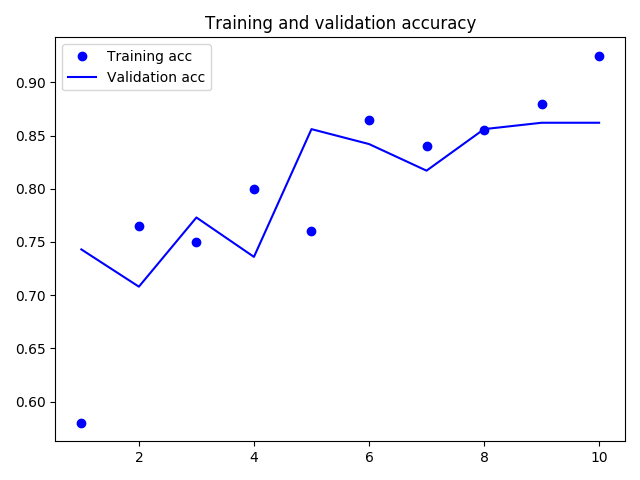
\includegraphics[scale=0.31]{images/machine_learning_accuracy.png} }}%
	\qquad
	\subfloat[]{{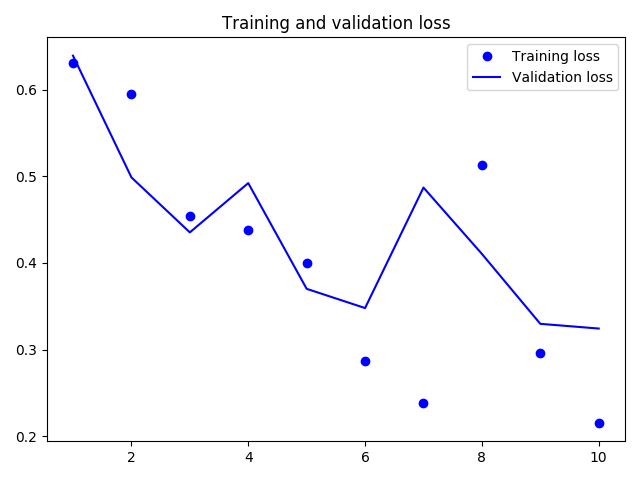
\includegraphics[scale=0.31]{images/machine_learning_acc.png} }}%
	\caption{
		Training and validation accuracy and loss when using pretrained word embeddings
	}
	\label{fig:example}
\end{figure}

After testing the algorithm in test data, the following results occurred with an accuracy of \textbf{85.36\%}, precision \textbf{78.15\%}, recall \textbf{88.90\%}, f1 score \textbf{82.61\%}. These results lead to a conclusion that LSTM-RNN algorithm seems to be more appropriate for argument mining problems, comparing to Random Forest and the Structural approach examined in the previous section.

\begin{lstlisting}[language=bash]
Found 10823 unique tokens.
Shape of data tensor: (5054, 235)
Shape of label tensor: (5054,)
Found 400000 word vectors.

Model: "sequential"
_________________________________________________________________
Layer (type)                 Output Shape              Param #   
=================================================================
embedding (Embedding)        (None, None, 100)         1000000   
_________________________________________________________________
lstm (LSTM)                  (None, 100)               80400     
_________________________________________________________________
dense (Dense)                (None, 1)                 101       
=================================================================
Total params: 1,080,501
Trainable params: 1,080,501
Non-trainable params: 0
_________________________________________________________________
None

Train on 200 samples, validate on 1000 samples
Epoch 1/10
200/200 [==============================] - 2s 10ms/sample - loss: 0.6307 - acc: 0.6350 - f1_m: 0.3386 - precision_m: 0.9722 - recall_m: 0.2519 - val_loss: 0.6393 - val_acc: 0.6090 - val_f1_m: 0.6948 - val_precision_m: 0.5351 - val_recall_m: 0.9980
Epoch 2/10
200/200 [==============================] - 2s 9ms/sample - loss: 0.5955 - acc: 0.6250 - f1_m: 0.4697 - precision_m: 0.7757 - recall_m: 0.5645 - val_loss: 0.4988 - val_acc: 0.8390 - val_f1_m: 0.8320 - val_precision_m: 0.7773 - val_recall_m: 0.8969
Epoch 3/10
200/200 [==============================] - 1s 7ms/sample - loss: 0.4542 - acc: 0.8700 - f1_m: 0.8178 - precision_m: 0.8778 - recall_m: 0.7895 - val_loss: 0.4353 - val_acc: 0.8150 - val_f1_m: 0.8213 - val_precision_m: 0.7220 - val_recall_m: 0.9551
Epoch 4/10
200/200 [==============================] - 1s 7ms/sample - loss: 0.4383 - acc: 0.8000 - f1_m: 0.7469 - precision_m: 0.8571 - recall_m: 0.7411 - val_loss: 0.4922 - val_acc: 0.7600 - val_f1_m: 0.7883 - val_precision_m: 0.6582 - val_recall_m: 0.9867
Epoch 5/10
200/200 [==============================] - 1s 7ms/sample - loss: 0.3999 - acc: 0.8250 - f1_m: 0.8295 - precision_m: 0.8415 - recall_m: 0.8676 - val_loss: 0.3702 - val_acc: 0.8500 - val_f1_m: 0.8494 - val_precision_m: 0.7830 - val_recall_m: 0.9289
Epoch 6/10
200/200 [==============================] - 1s 6ms/sample - loss: 0.2866 - acc: 0.9050 - f1_m: 0.8928 - precision_m: 0.8759 - recall_m: 0.9155 - val_loss: 0.3480 - val_acc: 0.8490 - val_f1_m: 0.8474 - val_precision_m: 0.7793 - val_recall_m: 0.9292
Epoch 7/10
200/200 [==============================] - 1s 7ms/sample - loss: 0.2383 - acc: 0.9050 - f1_m: 0.9028 - precision_m: 0.8486 - recall_m: 0.9646 - val_loss: 0.4870 - val_acc: 0.7960 - val_f1_m: 0.7277 - val_precision_m: 0.9137 - val_recall_m: 0.6066
Epoch 8/10
200/200 [==============================] - 1s 6ms/sample - loss: 0.5132 - acc: 0.7800 - f1_m: 0.7525 - precision_m: 0.7843 - recall_m: 0.8197 - val_loss: 0.4105 - val_acc: 0.8100 - val_f1_m: 0.7571 - val_precision_m: 0.8881 - val_recall_m: 0.6615
Epoch 9/10
200/200 [==============================] - 1s 6ms/sample - loss: 0.2962 - acc: 0.8850 - f1_m: 0.8746 - precision_m: 0.9322 - recall_m: 0.8448 - val_loss: 0.3297 - val_acc: 0.8650 - val_f1_m: 0.8500 - val_precision_m: 0.8417 - val_recall_m: 0.8593
Epoch 10/10
200/200 [==============================] - 1s 6ms/sample - loss: 0.2154 - acc: 0.9500 - f1_m: 0.9505 - precision_m: 0.9344 - recall_m: 0.9677 - val_loss: 0.3243 - val_acc: 0.8710 - val_f1_m: 0.8628 - val_precision_m: 0.8376 - val_recall_m: 0.8928
1264/1264 [==============================] - 1s 938us/sample - loss: 0.3474 - acc: 0.8536 - f1_m: 0.8261 - precision_m: 0.7815 - recall_m: 0.8890
Accuracy: 85.36%
Precision: 78.15%
Recall: 88.90%
F1 score: 82.61%
\end{lstlisting}

